\documentclass[a4paper,11pt]{article}
\usepackage[utf8]{inputenc}
\usepackage[T1]{fontenc}
\usepackage[polish]{babel}
\usepackage{graphicx}
\usepackage{booktabs}
\usepackage{geometry}
\usepackage{hyperref}
\geometry{margin=2.5cm}

\title{Projekt 6: Problem wieloagentowy\\środowisko CollectCoins}
\author{Szymon Kowalski \and Michał Król}
\date{\today}

\begin{document}
\maketitle

\section{Opis środowiska}

Zaimplementowaliśmy własne środowisko wieloagentowe \textbf{CollectCoins} w API PettingZoo (\texttt{ParallelEnv}).
Dwóch agentów (\texttt{agent\_0}, \texttt{agent\_1}) porusza się po dyskretnej siatce $9\times9$.
W każdym epizodzie pojawiają się cztery monety do zebrania w limicie 65 kroków.
Akcje: \emph{stay}, \emph{up}, \emph{down}, \emph{left}, \emph{right}.

Mapa zawiera stałe przeszkody (dwa słupy ścian), a obserwacja agenta obejmuje:
własną pozycję, pozycję partnera, współrzędne monet, ułamek czasu epizodu
oraz cztery sensory ścian (czy ruch w danym kierunku jest możliwy).

Nagroda: $+1$ za zebraną monetę (wspólna), niewielki \emph{shaping} za zbliżenie się do monety
oraz kara $-0{,}01$ za każdy krok.

\section{Zastosowane algorytmy}

Wykorzystaliśmy bibliotekę \textbf{Stable-Baselines3} (trening na CPU, polityka MLP $128\times128$):
\begin{itemize}
  \item \textbf{PPO} --- wariant \texttt{v0} (lr $=3\cdot10^{-4}$) oraz \texttt{v1} (lr $=10^{-3}$, większa entropia),
  \item \textbf{A2C} --- wariant \texttt{v0}.
\end{itemize}

\section{Eksperymenty}

\subsection{Ten sam algorytm (parameter sharing)}
Jeden model trenujemy na pojedynczym agencie (partner losowy), a w ewaluacji
\textbf{ten sam model} steruje oboma agentami na podstawie ich własnych obserwacji.

\subsection{Różne algorytmy w epizodzie}
\texttt{agent\_0} sterowany jest przez PPO, \texttt{agent\_1} przez A2C; oba modele grają wspólnie w jednym epizodzie.

Dla każdej konfiguracji wykonaliśmy 3 niezależne uruchomienia (seedy).
Budżet treningu: 200\,000 kroków (shared) lub $2\times100\,000$ (mixed).
Ewaluacja co 5\,000 kroków na 20 epizodach testowych.

\section{Wyniki i krzywe uczenia}

Tabela~\ref{tab:results} zestawia średnią nagrodę zespołu na początku i na końcu treningu
oraz wartość maksymalną na krzywej uczenia (uśrednione po seedach).

\begin{table}[h]
\centering
\caption{Podsumowanie krzywych uczenia (średnia nagroda zespołu).}
\label{tab:results}
\begin{tabular}{lccc}
\toprule
Konfiguracja & Początek & Koniec & Szczyt \\
\midrule
PPO v0 (shared) & +1.54 & +2.64 & +3.84 \\
PPO v1 (shared) & +1.65 & +2.74 & +3.69 \\
A2C (shared)    & +1.10 & +3.03 & +3.87 \\
Mixed PPO+A2C   & +2.73 & +4.08 & +4.08 \\
\bottomrule
\end{tabular}
\end{table}

Na wykresach widać wyraźny wzrost nagrody w trakcie uczenia.
Najwyższe wyniki osiąga konfiguracja mieszana (PPO + A2C), osiągając ok.\ $4.0$ nagrody/epizod
(przy maksymalnie ok.\ $4$ monetach plus shaping).

\begin{figure}[h]
\centering
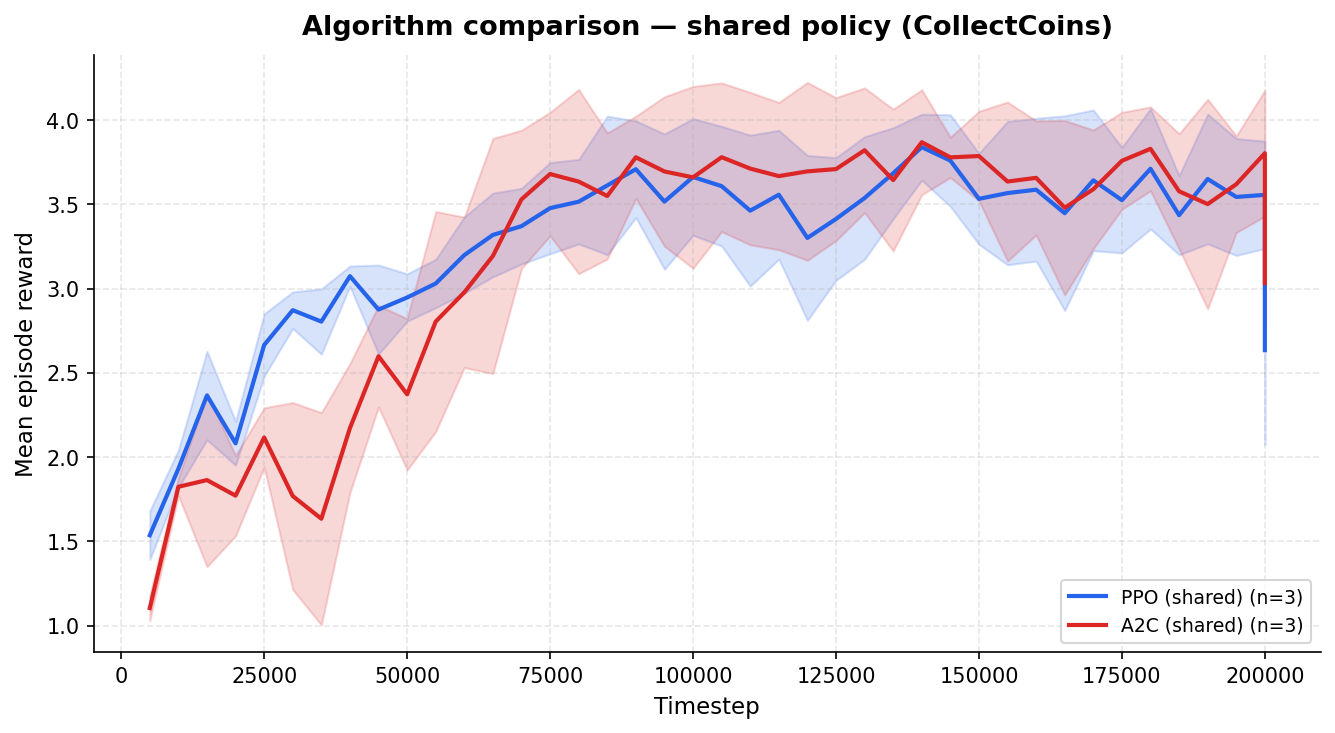
\includegraphics[width=0.95\linewidth]{../plots/algo_comparison.png}
\caption{Porównanie algorytmów PPO i A2C (ten sam algorytm, parameter sharing).}
\end{figure}

\begin{figure}[h]
\centering
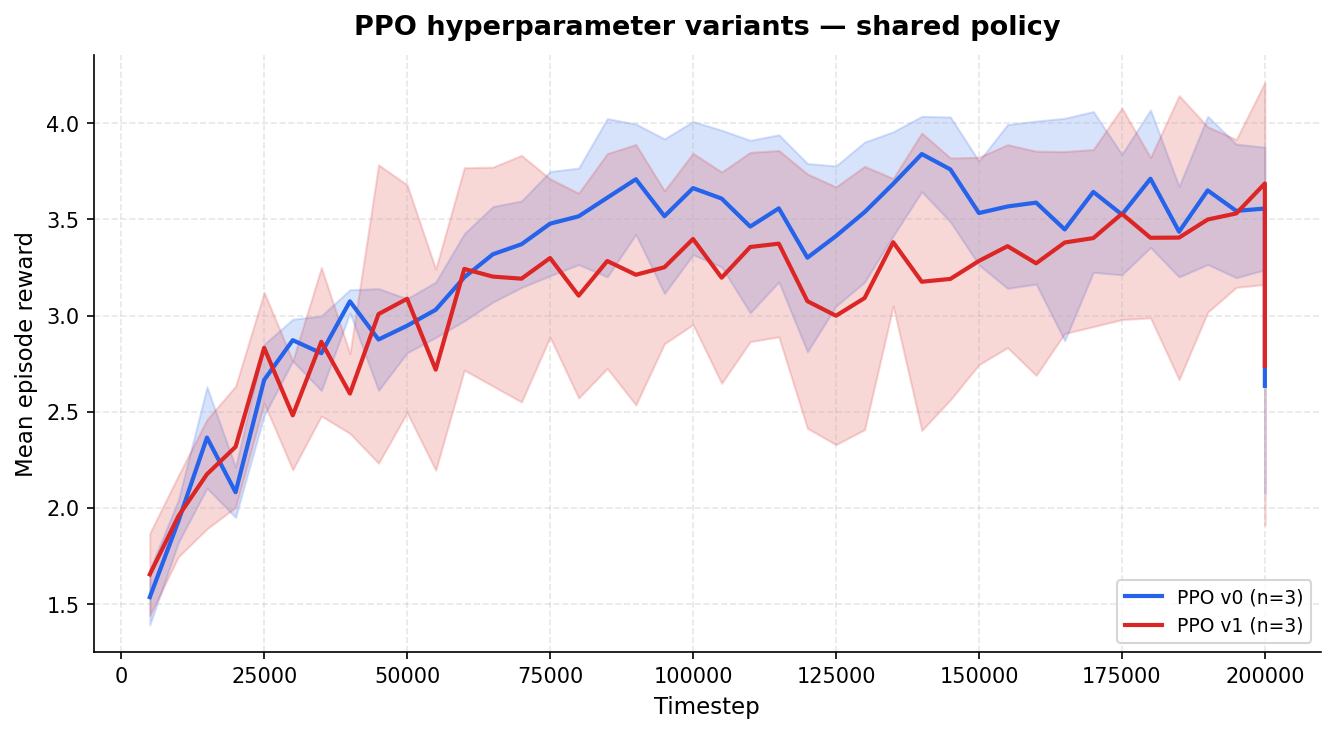
\includegraphics[width=0.95\linewidth]{../plots/ppo_variants.png}
\caption{Porównanie wariantów hiperparametrów PPO (v0 vs v1).}
\end{figure}

\begin{figure}[h]
\centering
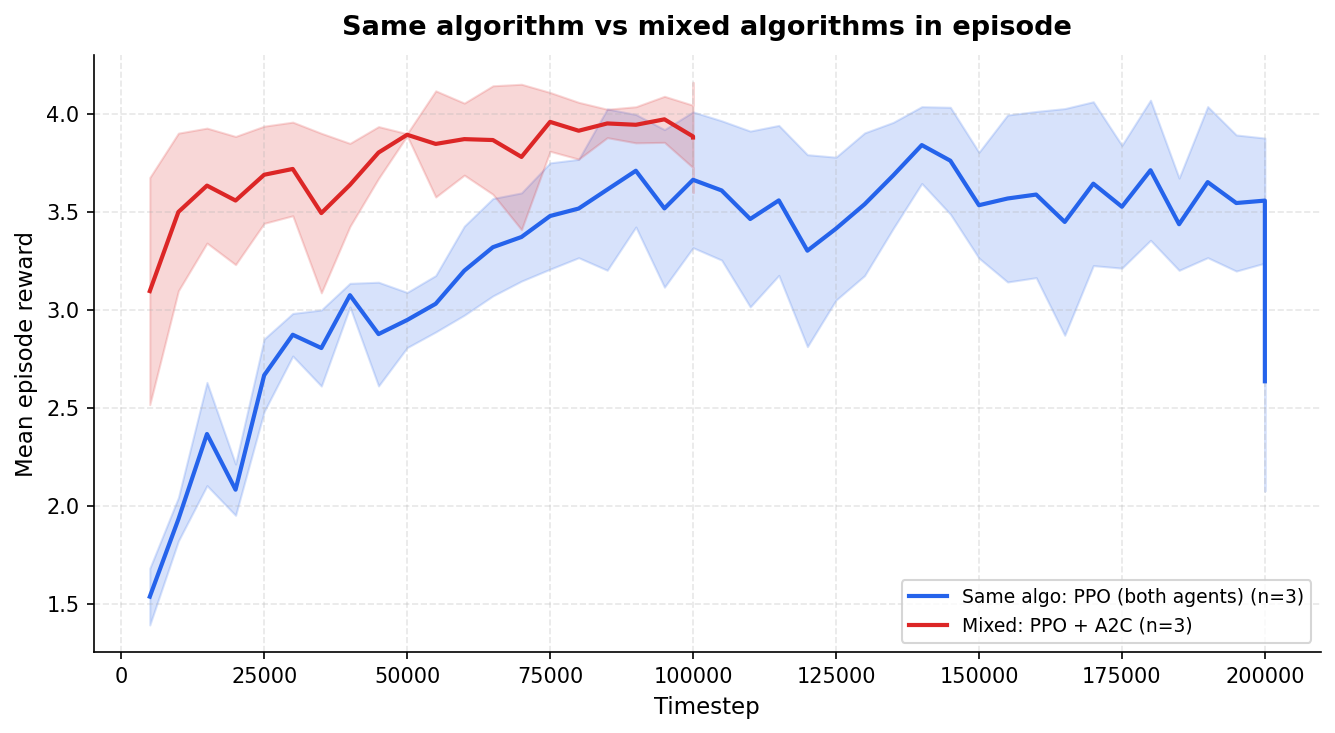
\includegraphics[width=0.95\linewidth]{../plots/same_vs_mixed.png}
\caption{Ten sam algorytm (PPO) vs różne algorytmy w epizodzie (PPO + A2C).}
\end{figure}

\section{Wnioski}

\begin{itemize}
  \item Agenci uczą się zbierać monety we współpracy --- krzywe uczenia rosną z ok.\ $1$--$1.5$
        do ok.\ $3$--$4$ nagrody zespołu.
  \item \textbf{A2C} osiąga porównywalne wyniki do PPO w trybie shared, przy nieco większej zmienności.
  \item Wariant PPO z wyższym learning rate (v1) uczy się szybciej na początku, lecz końcowa jakość
        jest zbliżona do wariantu domyślnego.
  \item Konfiguracja \textbf{mixed} (różne algorytmy) osiąga najlepsze wyniki końcowe,
        co sugeruje, że specjalizacja agentów (PPO + A2C) może pomóc w koordynacji.
  \item Stała mapa ze ścianami i sensory w obserwacji są istotne dla stabilnego uczenia ---
        wcześniejsze próby z losowymi ścianami bez pełnej obserwacji dawały słabe wyniki.
\end{itemize}

\section{Uruchomienie}

Kod projektu: \texttt{project06/}. Trening: \texttt{python -m project06.train\_shared},
\texttt{python -m project06.train\_mixed}. Wykresy: \texttt{python -m project06.plot}.
Wizualizacja epizodu: \texttt{python -m project06.visualize}.

\end{document}
